\documentclass{article}
\usepackage[utf8]{inputenc}

\usepackage{geometry}
\usepackage{bm}
\geometry{a4paper}
\usepackage{latexsym}
%\usepackage[dvips]{graphicx}
\usepackage{epsfig}
\usepackage{amsmath}
\usepackage{amsfonts}
\usepackage{amssymb}
\usepackage{eucal}
\usepackage{mathrsfs}
\usepackage{wasysym}
\usepackage{setspace}
\usepackage{float}
\usepackage{color}
\usepackage{rotating}
\usepackage{stmaryrd}
\usepackage{lineno}

\numberwithin{equation}{section}
\frenchspacing
%%
\usepackage{amsthm}


%%%%INSERITI ADESSO%%%%
\usepackage{amsmath}
\usepackage{amsfonts}
\usepackage{amssymb}
\usepackage{amsthm}
\usepackage{mathrsfs}
\usepackage{eucal}  
\theoremstyle{definition}
\usepackage{accents}
\usepackage{array}
\usepackage{cases}
\usepackage{graphicx}
\usepackage{booktabs}
\usepackage{caption}
\usepackage{cancel}
\usepackage{bbm}
\usepackage{subfig}
\usepackage{enumitem}
\usepackage{movie15}
 \usepackage{algorithm}
\usepackage{algpseudocode}
\usepackage{tabularx}
\usepackage{longtable}
 
% Font Management
\usepackage[T1]{fontenc}       % 8 bit font encoding: includes all accents
\usepackage{bm}                % alternative to \bs provided by package amsmath
\usepackage{bbm}               % alternative to \mathbb;  usage: \mathbbm{}
%\usepackage[mathscr]{eucal}    % alternative to \mathcal; usage: \mathcal{}
\usepackage{color}             % for text in colour
\usepackage{verbatim}          % environment for commenting out blocks of text
%\usepackage{exscale}           % needed to scale cmdx fonts
%\usepackage{ae,aecompl}        % see http://www.ctan.org/tex-archive/fonts/ae
%%%%%%%%%%%%%%%%%%


\theoremstyle{plain}
\newtheorem{thm}{Theorem}[section]
\newtheorem{lem}[thm]{Lemma}
\newtheorem{prop}[thm]{Proposizione}
\newtheorem*{cor}{Corollario}

\theoremstyle{definition}
\newtheorem{defn}{Definizione}[section]
\newtheorem{conj}{Congettura}[section]
\newtheorem{exmp}{Esempio}[section]

\theoremstyle{remark}
\newtheorem*{rem}{Osservazione}
\newtheorem*{note}{Nota}

\DeclareMathOperator*{\argmin}{argmin}
\DeclareMathOperator*{\argmax}{argmax}

\newcommand{\dom}{\mathrm{dom}}
\newcommand{\im}{\mathrm{im}}
\newcommand{\sign}{\mathrm{sign}}
\newcommand{\abs}{\mathrm{abs}}
\newcommand{\e}{\mathrm{exp}}

\setlength{\textwidth}{15 cm}
\setlength{\textheight}{23.5 cm}



%%%%%%%%%%%%%%%%%%%%%%%%%%%%%%%%%%%%%%%%%%%%%%%%%%%

\usepackage[utf8]{inputenc}
\usepackage[T1]{fontenc}
\usepackage{lmodern}

\usepackage{hyperref}
\hypersetup{%
    pdfpagemode={UseOutlines},
    bookmarksopen,
    pdfstartview={FitH},
    colorlinks,
    linkcolor={blue},
    citecolor={blue},
    urlcolor={blue}
  }

%%%%%%% use PDFLATEX 

\usepackage{lipsum} %to insert random text

\usepackage{geometry} %for the margins
\newcommand\fillin[1][4cm]{\makebox[#1]{\dotfill}} %for the dotted line in the frontispiace

\usepackage{dcolumn}
\newcolumntype{d}{D{.}{.}{-1} } %to vetical align numbers in tables, along the decimal dot

\usepackage{amsmath}



%%%%%%% Local definitions
\newtheorem{osservazione}{Osservazione}% Standard LaTeX
\newtheorem{observation}{Observation}% Standard LaTeX

\newcommand{\BR}{\mathscr{B}_{\mathrm{R}}}
\newcommand{\T}[2]{T_{#2}#1}
\newcommand{\cT}[2]{T_{#2}^{*}#1}
\newcommand{\pder}[2]{\frac{\partial #1}{\partial #2}}

				 
%%%%%%%%%%%%%%%%%%%%%%%%%%%%%%%%%%%%%%%%%%%%%%%%%
%
% Inserito il codice Matlab
%
\usepackage{listings}
\usepackage{hyperref}
\usepackage{xcolor}
\lstset{
backgroundcolor=\color{white},   
basicstyle=\footnotesize\ttfamily,        
breakatwhitespace=true,         % sets if automatic breaks should only happen at whitespace
breaklines=true,                 % sets automatic line breaking
captionpos=b,                    % sets the caption-position to bottom
commentstyle=\color{gray},                
keepspaces=true,                 % keeps spaces in text, useful for keeping indentation of code
columns=flexible,
keywordstyle=\color{blue},       % keyword style
language=MATLAB,                 % the language of the code
morekeywords={*,...},            % if you want to add more keywords to the set
deletekeywords={gamma,beta},
numbers=left,                    % where to put the line-numbers; possible values are (none, left, right)
numbersep=10pt,                   % how far the line-numbers are from the code
numberstyle=\tiny\color{gray}, % the style that is used for the line-numbers
rulecolor=\color{black},         % if not set, the frame-color may be changed on line-breaks within not-black text (e.g. comments (green here))
showspaces=false,                % show spaces everywhere adding particular underscores; it overrides 'showstringspaces'
showstringspaces=false,          % underline spaces within strings only
showtabs=false,                  % show tabs within strings adding particular underscores
stepnumber=1,                    % the step between two line-numbers. If it's 1, each line will be numbered
tabsize=2,	                   % sets default tabsize to 2 spaces
frame=lines,                   %POSSO TOGLIERLO
} 



\title{Computational Linear Algegbra For Large Scale Problems}
\author{Nenna Giulio, Ornella Elena Grassi}
\date{Spectral Clustering Homework}
\begin{document}
\maketitle
The aim of this homework is to implement and apply \textbf{Spectral Clustering} to two different sets of datapoints in \(\mathbb{R}^2\). The two sets are shown in Figure \ref{scatter_intro}
\begin{figure}[H]
  \centering
  \subfloat[1][Scatterplot of the data stored in \texttt{Circle.mat}]{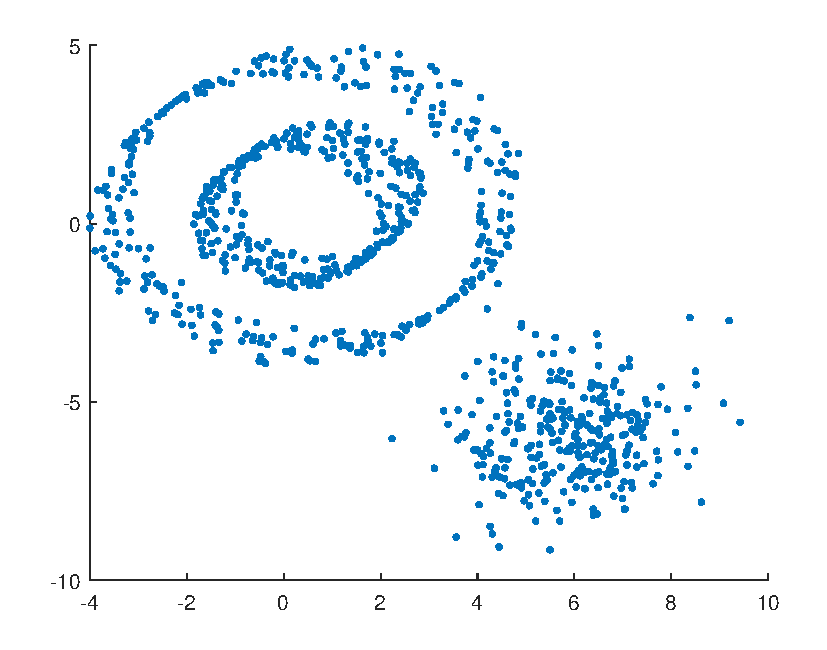
\includegraphics[scale = 0.45]{pictures/circle_scatterplot.pdf}}
  \qquad
  \qquad
  \subfloat[2][Scatterplot of the data stored in \texttt{Spiral.mat}]{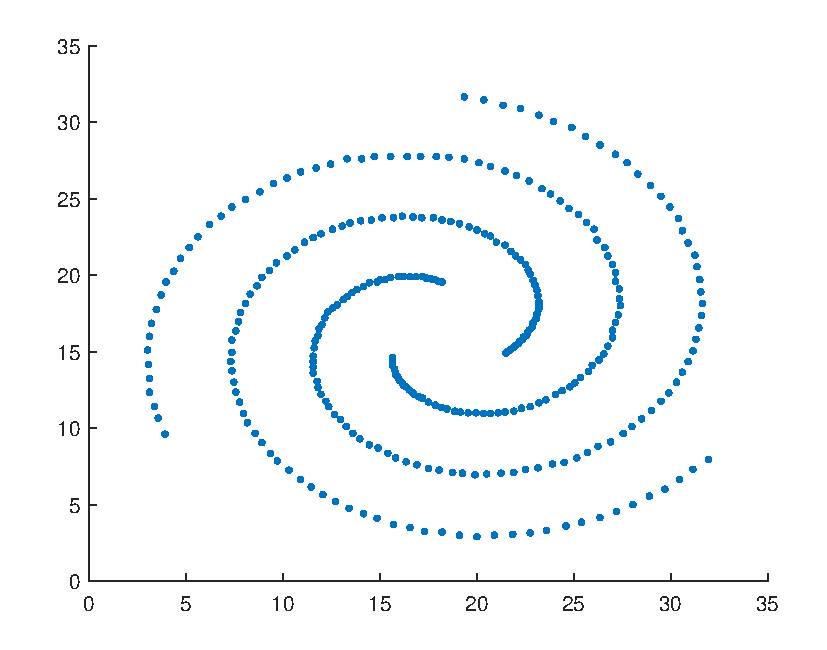
\includegraphics[scale = 0.45]{pictures/spiral_scatterplot.pdf}}
  \caption{Scatterplot of the two Datasets}
  \label{scatter_intro}
\end{figure}

As it is clearly visible through visual inspection, both datasets contain \(3\) different shapes that can be classified as different clusters. In the \texttt{Circle} dataset there are two concentrical circles and a cloud of points in the bottom right while in the \texttt{Spiral} dataset there are 3 spirals. Traditional clustering algorithms, that mainly rely on euclidean distance, may fail in recognizing the presence of shapes in our data hence our need to rely on a different technique called \textbf{Spectral clustering}. 
\\
\\

\section{K-Nearest Neighborhood Graph}
First, we need to define a similarity function that measures "how much our points are similar to each other". Let \(X_i\) and \(X_j\) be two points in our data, then we will use a similarity measure defined as:
\begin{equation}
  s_{i,j} = \exp \left(- \frac{\| X_i- X_j \|^2}{2\sigma^2}\right)
\end{equation}
Then, a \textit{\(K\)-Nearest Neighborhood} similarity graph is a Graph \(G= (V,E)\) where each vertex \(v_1, \dots v_n\) represents a point and two vertices \(v_i\) and \(v_j\) are connected by an undirected edge \(e_{i,j}\) if the similarity between \(v_i\) and \(v_j\) is among the \(K\)-th highest similarities between \(v_i\) and other vertices in \(V\). For such graph we can define the relative adjacency matrix as \(W_{i,j} = s_{i,j}\) where each entry \(W_{i,j}\) is nonzero only if there exists an edge between \(v_i\) and \(v_j\). \(W\) has zero-values on the diagonal by definition.
\\
\\
The following MATLAB code was use to generate the K-NN similarity graph of our data:
\lstinputlisting{../knn_graph.m}
Running \texttt{knn\_graph} on both dataset using \(\sigma= 1\) and testing with \(K= 10, 20, 40\) gave the following results:
\begin{figure}[H]
  \centering
  \subfloat[1][\(K= 10\)]{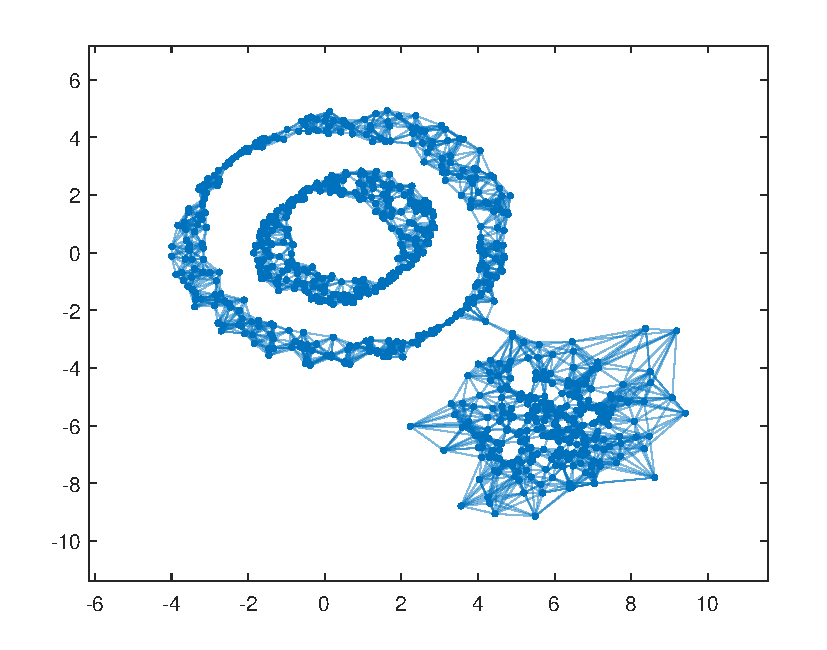
\includegraphics[scale = 0.37]{pictures/circle_KNN_K10.pdf}}
  \subfloat[2][\(K= 20\)]{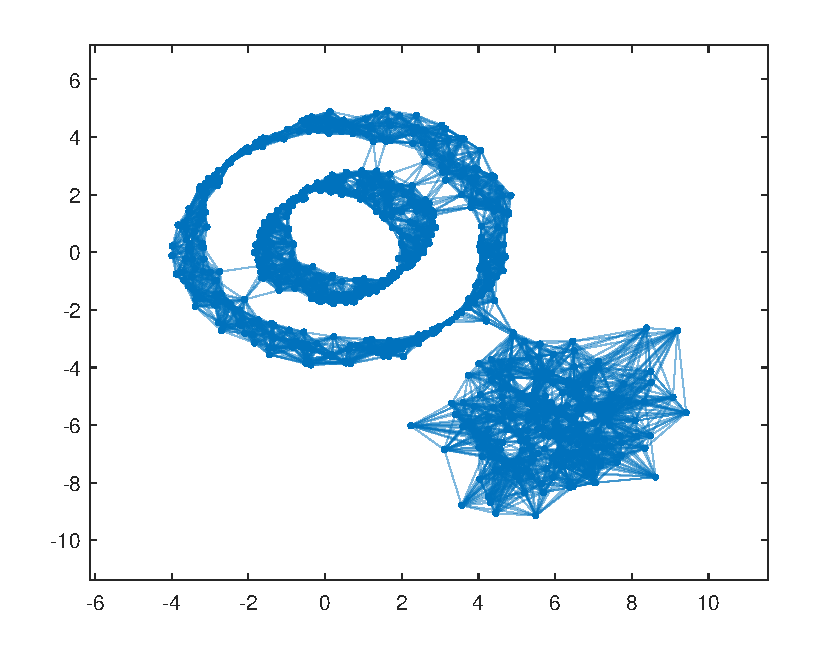
\includegraphics[scale = 0.37]{pictures/circle_KNN_K20.pdf}}
  \subfloat[3][\(K= 40\)]{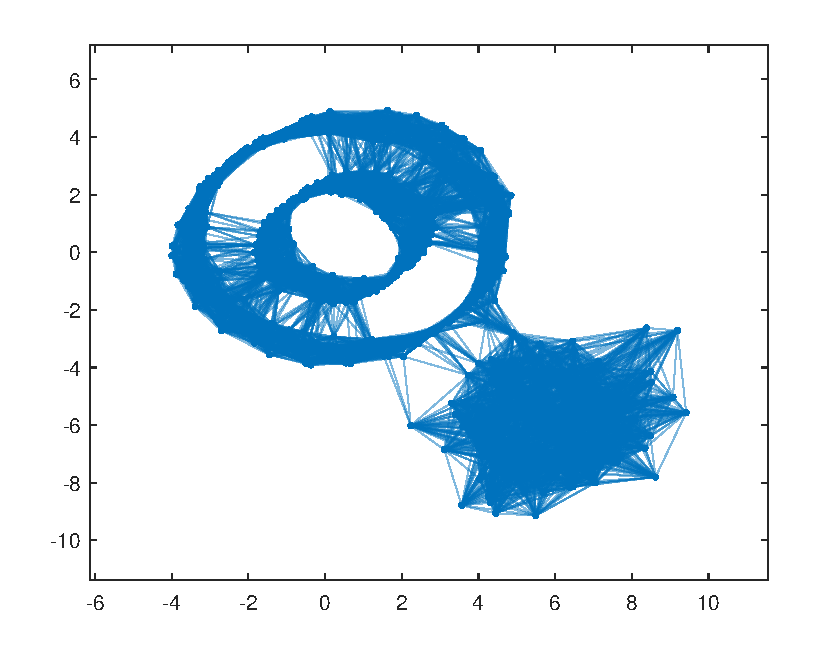
\includegraphics[scale = 0.37]{pictures/circle_KNN_K40.pdf}}
  \caption{K-NN graphs plots for \texttt{Circle} data with different values of \(K\)}
  \label{KNN_circle}
\end{figure}
\begin{figure}[H]
  \centering
  \subfloat[1][\(K= 10\)]{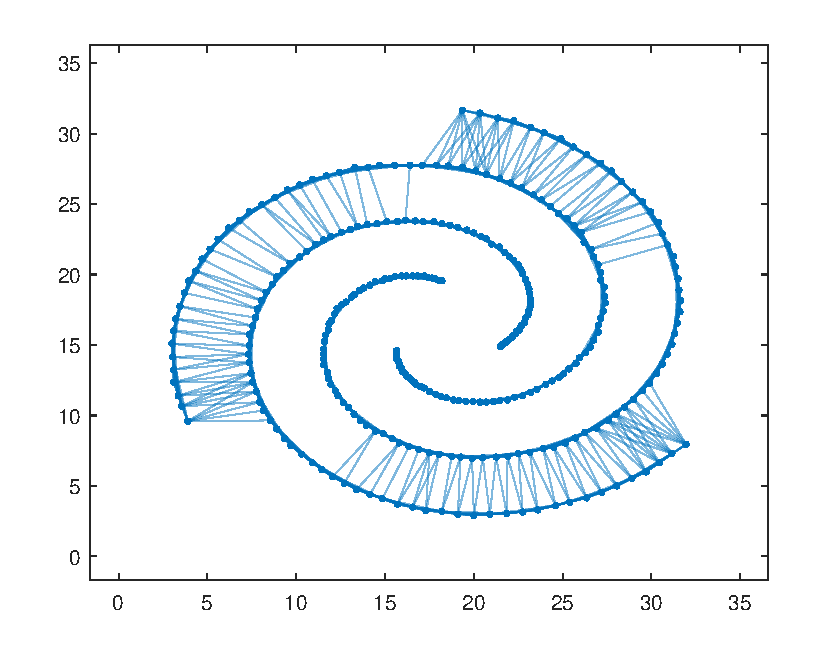
\includegraphics[scale = 0.37]{pictures/spiral_KNN_K10.pdf}}
  \subfloat[2][\(K= 20\)]{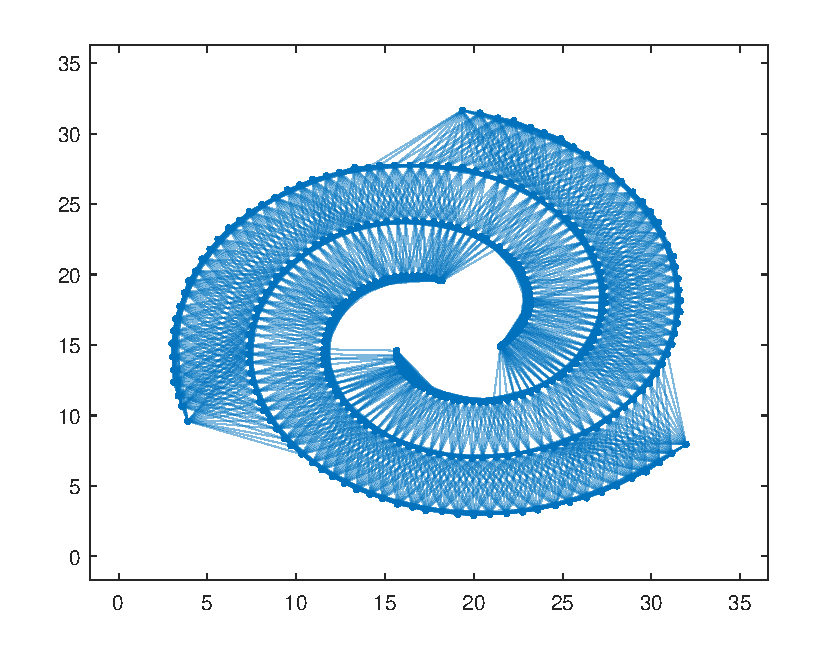
\includegraphics[scale = 0.37]{pictures/spiral_KNN_K20.pdf}}
  \subfloat[3][\(K= 40\)]{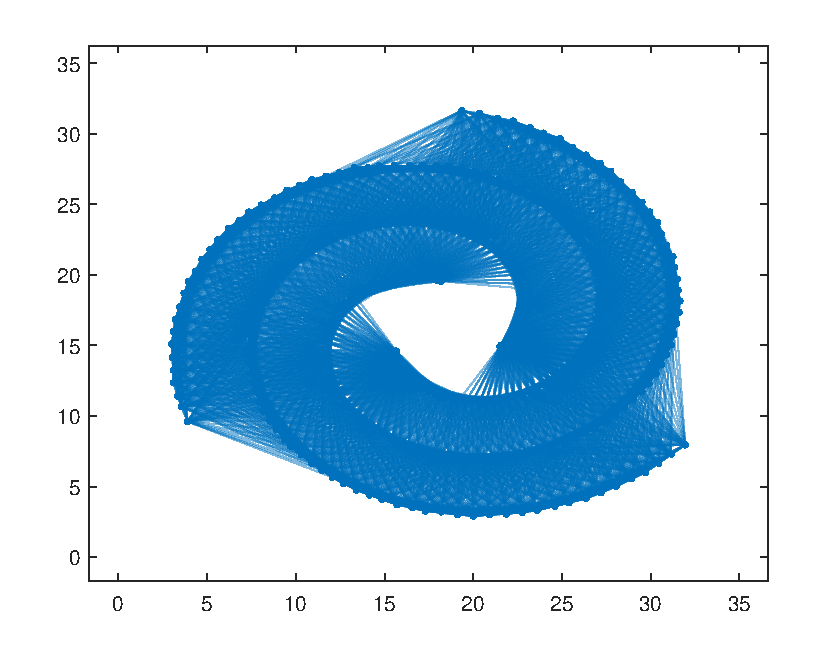
\includegraphics[scale = 0.37]{pictures/spiral_KNN_K40.pdf}}
  \caption{K-NN graphs plots for \texttt{Spiral} data with different values of \(K\)}
  \label{KNN_spiral}
\end{figure}

Our objective is to find a K-NN graph that "separates well" the shapes, meaning that in the best case each shape is a connected component of the graph. As we can see, for both \texttt{Circle} and \texttt{Spiral} data, the value \(K = 10\) seems to separate the shapes well. We will quantify the concept of \textit{good cluster separation} in the next section.
\section{Degree and Laplacian Matrices}
\label{sec2}
The \textit{Degree matrix} \(D\) is a diagonal matrix that has the degree of each node on the diagonal where the degree of a node \(v_i\) is the sum of the weights of all the edges that are connected to such node. Since in our case edge weights correspond to similarities, the degree of each node is the sum of the similarities with all of its neighbors. This can be simply achieved with the following:
\begin{equation}
    D = \text{diag}(W \mathbbm{1})
\end{equation}
Since the Laplacian matrix is defined as \(L= D - W\), we use the following code to compute both \(D\) and \(L\):
\lstinputlisting{../graph_laplacian.m}
After computing both matrices for each dataset and for each value of \(K\) we are testing for the K-NN graph we can inspect each Laplacian matrix using the \texttt{spy} command in MATLAB:
\begin{figure}[H]
    \centering
    \subfloat[1][\(K= 10\)]{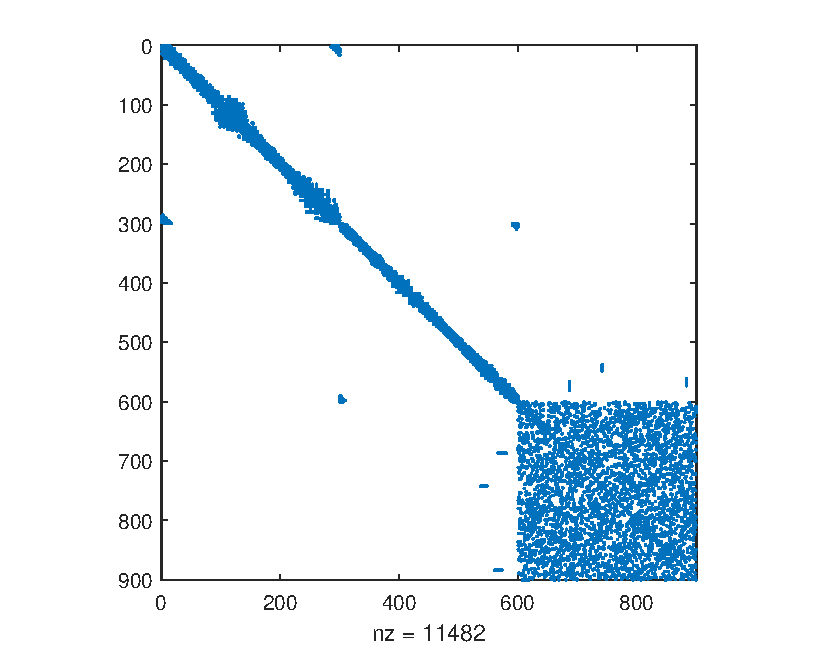
\includegraphics[scale = 0.37]{pictures/circle_LaplacianSpy_K10.pdf}}
    \subfloat[2][\(K= 20\)]{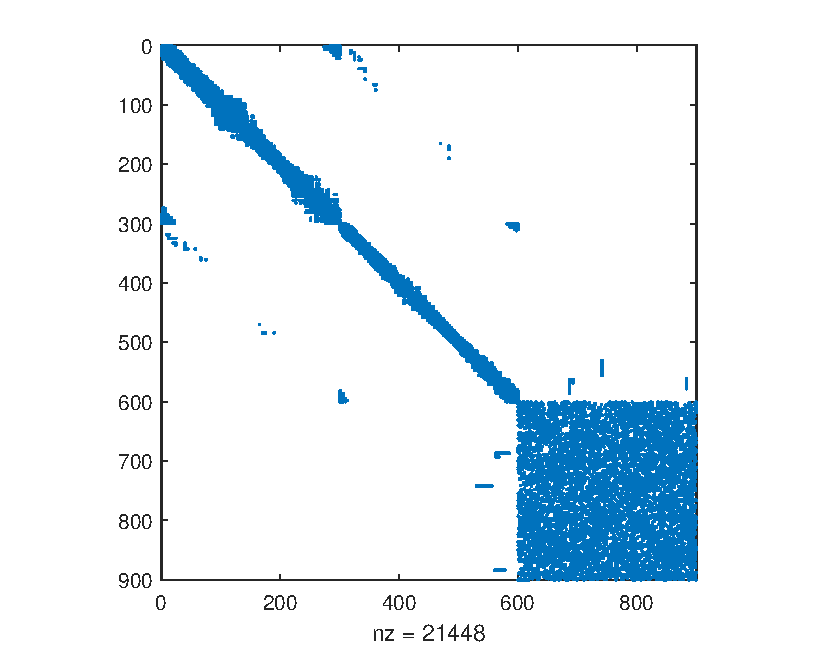
\includegraphics[scale = 0.37]{pictures/circle_LaplacianSpy_K20.pdf}}
    \subfloat[3][\(K= 40\)]{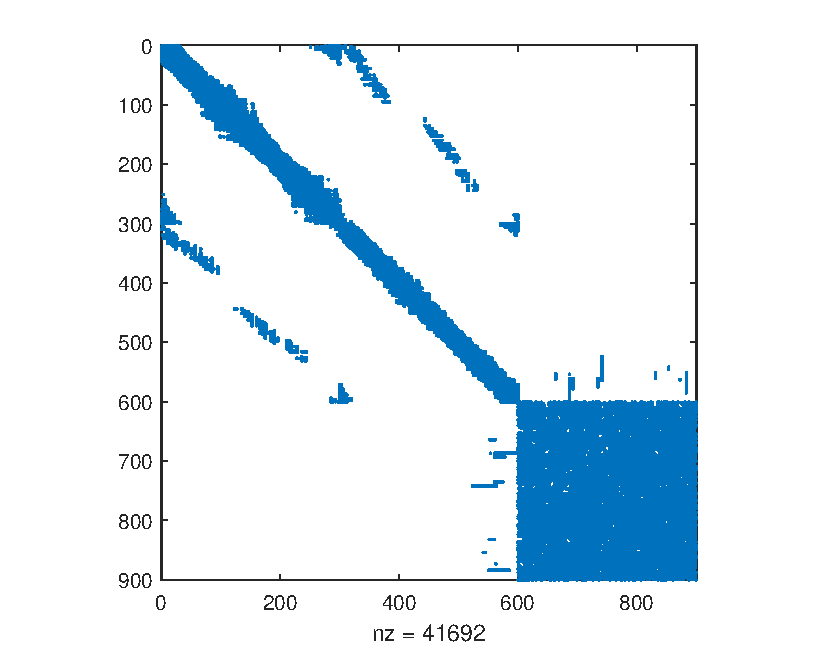
\includegraphics[scale = 0.37]{pictures/circle_LaplacianSpy_K40.pdf}}
    \caption{\texttt{spy} plots of the Laplacian matrix for \texttt{Circle} data with different values of \(K\)}
    \label{LaplacianSpy_circle}
  \end{figure}
  In Figure \ref{LaplacianSpy_circle} we can see that, for each Laplacian matrix inspected, there are 3 sections. Each section defines a "\textit{shape cluster}" in the \texttt{Circle} dataset: the first one is clearly visible in the bottom right corner of each matrix and it is relative to the point cloud. The other two sections are along the diagonal in the top left of the matrix, they are somewhat visible for \(K= 10\) and \(K= 20\) and they are relative to the two "circles" visible in the scatterplot in Figure \ref{scatter_intro}. The Laplacian matrix inspected for \(K= 40\) clearly shows a sort of \textbf{data pollution} from one shape cluster to another, this might suggest that the value \(K= 40\) may be too high for deploying the clustering.
  \begin{figure}[H]
    \centering
    \subfloat[1][\(K= 10\)]{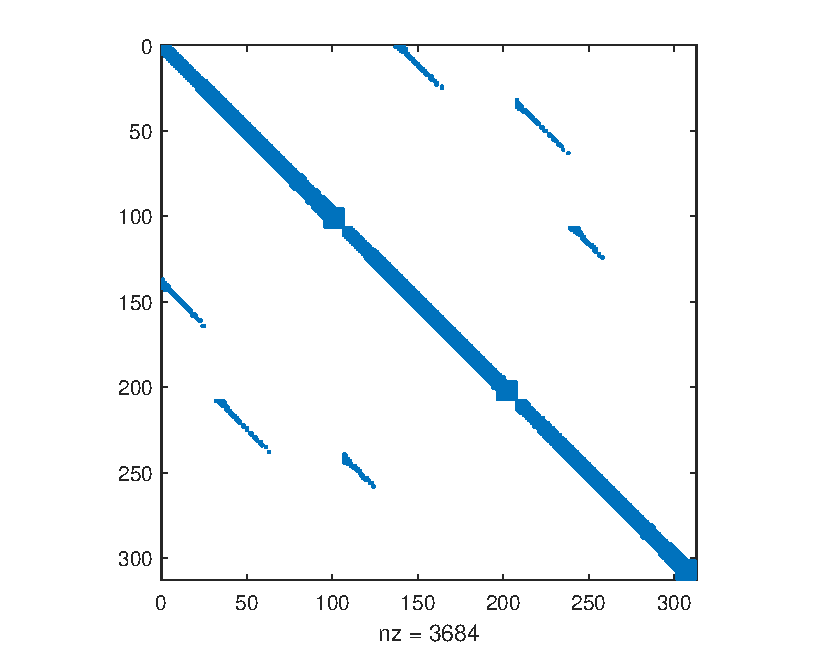
\includegraphics[scale = 0.37]{pictures/spiral_LaplacianSpy_K10.pdf}}
    \subfloat[2][\(K= 20\)]{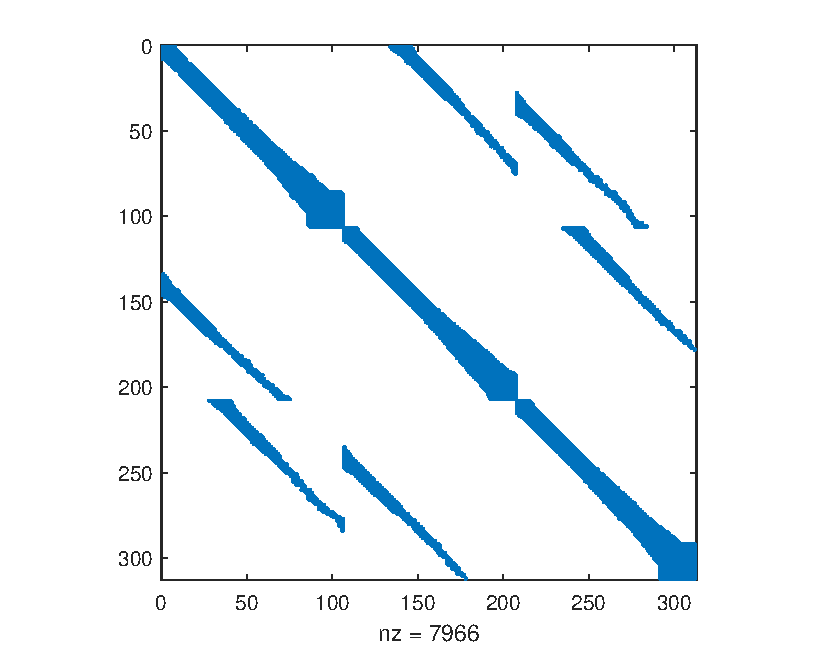
\includegraphics[scale = 0.37]{pictures/spiral_LaplacianSpy_K20.pdf}}
    \subfloat[3][\(K= 40\)]{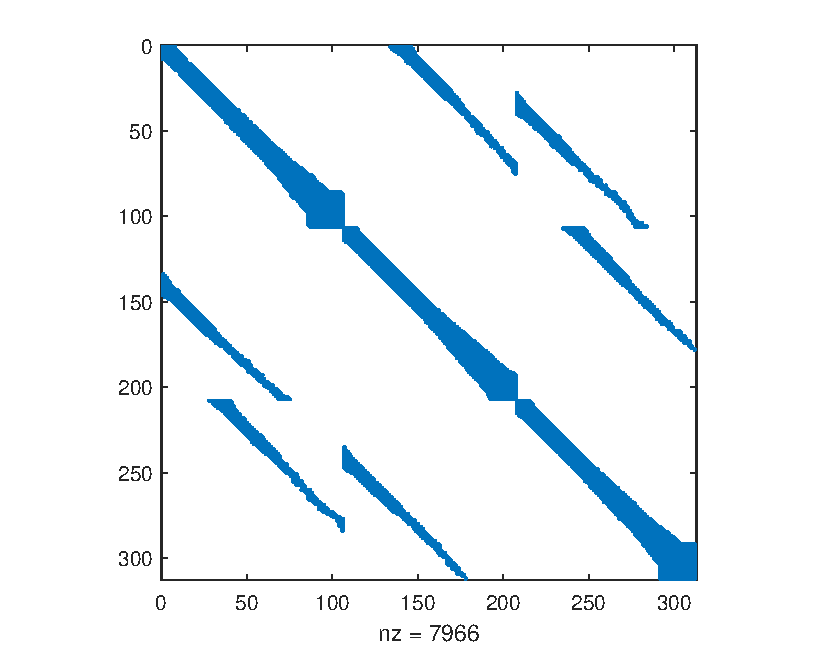
\includegraphics[scale = 0.37]{pictures/spiral_LaplacianSpy_K20.pdf}}
    \caption{\texttt{spy} plots of the Laplacian matrix for \texttt{Spiral} data with different values of \(K\)}
    \label{LaplacianSpy_spiral}
  \end{figure}
  The same concept can be applied for Figure \ref{LaplacianSpy_spiral}. Along the diagonal, three sections are visible and they represent the three different spirals seen in Figure \ref{scatter_intro}. As for \texttt{Circle} data, the KNN graph computed on the \texttt{Spiral} data with \(K= 40\) shows pollution between each spiral and this is visibile since there are a lot of non-zero elements away from the diagonal.
  \\
\\
The recurrent theme for both dataset is that the more \(K\) is higher, the more each shape will "pollute" another. This means that the corresponding Laplacian matrix will show a \textbf{lot of non-zero elements away from the diagonal} and this is a phenomenon that can (and will) impact computational costs.
\section{Connected components computation}
In order to compute the number of connected components in each graph we use the following result:
\begin{thm}
    Let \(G = (\mathcal{V}, W)\) be a finite graph and let \(L\) be its laplacian matrix. Then \(L\) has \(\lambda = 0\) as an eigenvalue and its algebraic multiplicity correspond to the number of connected components in \(G\).
\end{thm}
%\\
\noindent Using the Matlab function \texttt{eigs} we can compute the smallest \(C = 6\) eigenvalues of both graphs laplacian matrices \(L\) and for each value of \(K\) obtaining the following results:

\begin{center}
    \begin{table}[h!]
        \centering
        \begin{tabular}{|l|c|r|}
            \hline
            $K=10$ & $K=20$ & $K=40$ \\
            \hline
            8.5482e-17 & 2.4854e-16 & 8.1617e-16\\ 
            \hline
            3.7050e-16 & 0.0111 & 0.0482\\
            \hline
            0.0048 & 0.0652 & 0.7028\\
            \hline
            0.0286 & 0.1620 & 0.7797\\
            \hline
            0.0425 & 0.1724 & 0.9065\\
            \hline
            0.0429 & 0.3220 & 1.376\\
            \hline
        \end{tabular}
        \caption{Smallest 6 eigenvalues of the Laplacian matrix for the \texttt{circle} dataset}    
        \label{table_circle_spiral}
    \end{table}
    \begin{table}[h!]
        \centering
        \begin{tabular}{|l|c|r|}
            \hline
            $K=10$ & $K=20$ & $K=40$ \\
            \hline
            1.0496e-16 & 1.7853e-16 & 4.0554e-16\\
            \hline
            1.9667e-04 & 0.0018 & 0.0023\\
            \hline
            2.7219e-04 & 0.0020 & 0.0025\\
            \hline
            0.0041 & 0.0048 & 0.0049\\
            \hline
            0.0044 & 0.0054 & 0.0062\\
            \hline
            0.0046 & 0.0056 & 0.0067\\
            \hline
        \end{tabular}
        \caption{Smallest 6 eigenvalues of the Laplacian matrix for the \texttt{spiral} dataset} 
        \label{table_eigs_spiral}   
    \end{table}
\end{center}
From a visual inspection of both dataset we would expect to find 3 connected components and consequently an eigenvalue \(\lambda= 0\) of both laplacian matrices with algebraic multiplicity \(M= 3\).
\\
\\
Considering the case \(K= 10\) for both datasets we can see that the first 3 eigenvalues are "almost" equal to 0, and we can see a jump in order of magnitude from the fourth eigenvalue.
On the other hand the cases \(K=20\) and \(K=40\) show that only the first eigenvalue could be considered equal to 0 (which is always true) but the second and third eigenvalues are somewhat smaller than the others.
\\
This behaviour is perfectly in line with the "data pollution" concept seen graphically in \ref{sec2}. We can in fact interpret an "almost null" eigenvalue as an eigenvalue corresponding to an "almost connected component". The less the component is "isolated", the greater its eigenvalue will be. In the case \(K=10\) we clearly have 3 connected components that are isolated fairly well, hence the value of the first 3 eigenvalues are almost 0 for both graphs. In the cases \(K=20\) and \(K=40\), the 3 connected components that we expected are not well isolated and present a lot of edges from one to another, hence the first 3 eigenvalues are not small enough to be considered null.\\
\\
In any case we consider \(M=3\) the number of connected components and construct the matrix \(U\in \mathbb{R}^{N\times 3}\) using the \(M=3\) eigenvectors \(u_1, u_2, u_3\) corresponding to the first 3 eigenvalues as columns.
\\
\\
The following Matlab code was used for the computation in this section:
\lstinputlisting{../task3_4_5.m}
\section{Performing Spectral Clustering}
After computing the matrix \(U\in \mathbb{R}^{N\times3}\) for both the \texttt{circle} and the \texttt{spiral} datasets and for each \(K \in \{10, 20, 40\}\) we can now finally deploy a clustering algorithm.
\\
\\
Let \(y_i\in \mathbb{R}^M\) be the vector corresponding to the \(i\)-th row of the matrix \(U\). Then we can use the \textit{K-Means} algorithm to cluster the points \(y_i\), \(i \in \{1, \dots, N\}\) into \(M\) clusters and assign the original datapoints to the same cluster as their corresponding rows in \(U\). 
\\
\\
The following code was used in order to perform clustering:
\lstinputlisting{../task6_7_8.m}
Hence for both dataset we obtain 3 different clusterings, one for each value of \(K\) tested. Plotting the results we obtain:
\begin{figure}[H]
    \centering
    \subfloat[1][\(K= 10\)]{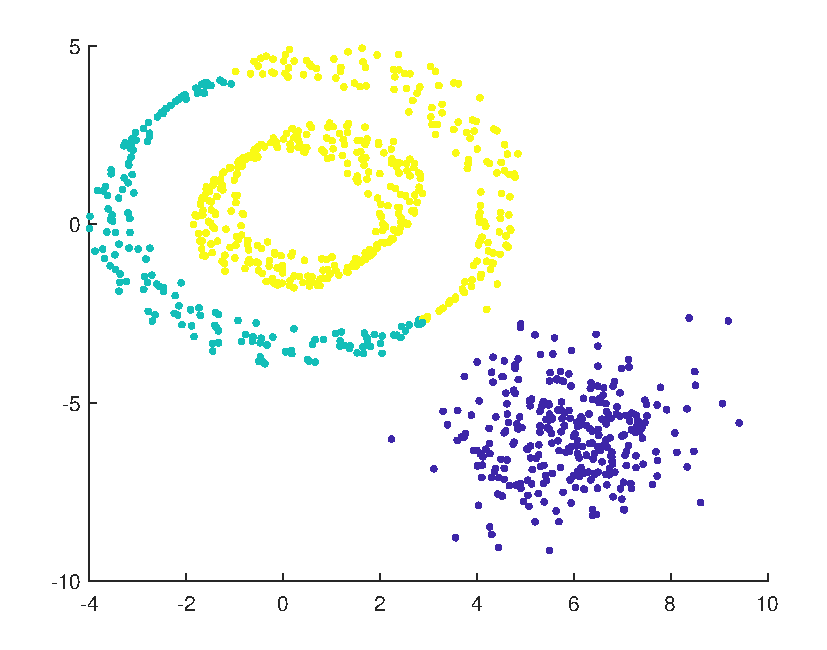
\includegraphics[scale = 0.37]{pictures/circle_SpectralClustering_K10.pdf}}
    \subfloat[2][\(K= 20\)]{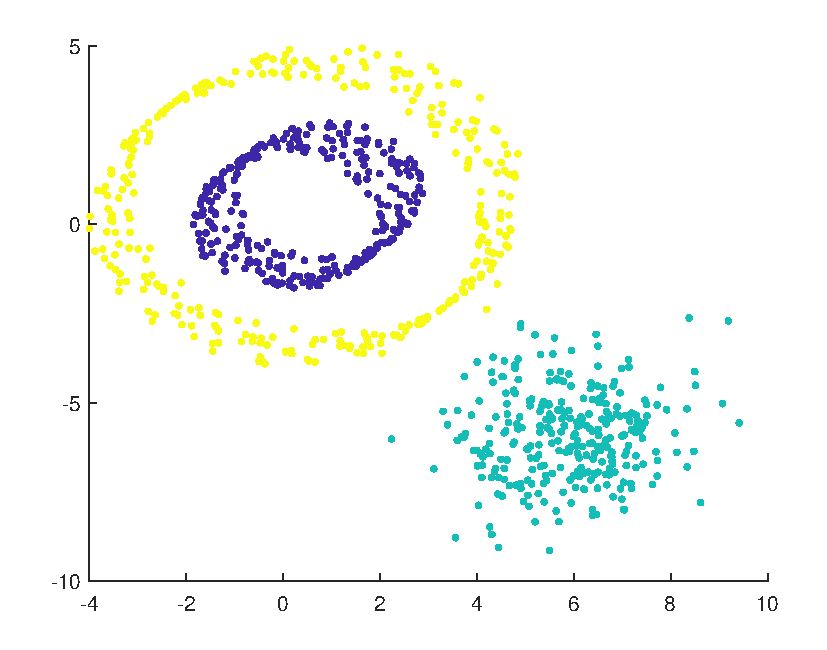
\includegraphics[scale = 0.37]{pictures/circle_SpectralClustering_K20.pdf}}
    \subfloat[3][\(K= 40\)]{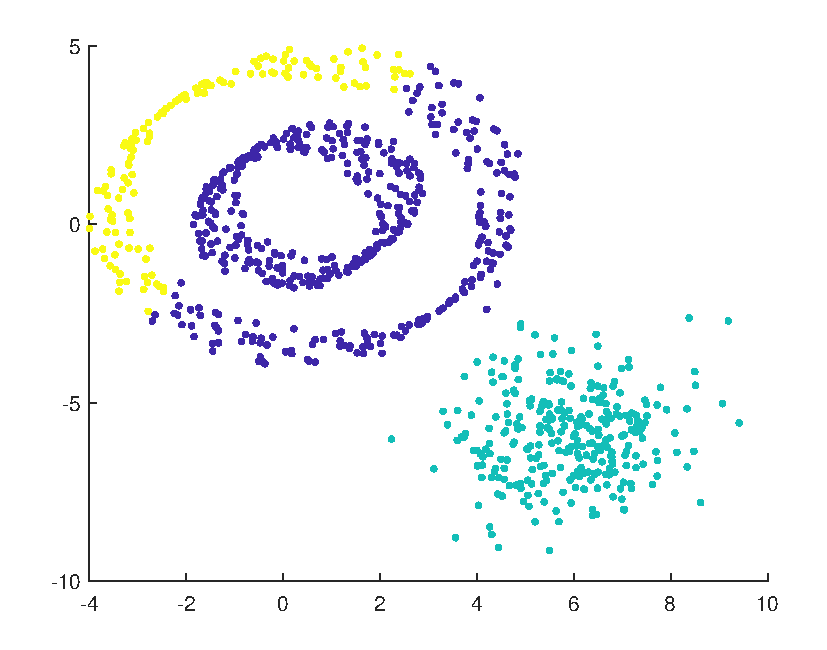
\includegraphics[scale = 0.37]{pictures/circle_SpectralClustering_K40.pdf}}
    \caption{Spectral clustering for \texttt{circle} data with different values of \(K\)}
    \label{spectral_circle}
  \end{figure}
  \begin{figure}[H]
    \centering
    \subfloat[1][\(K= 10\)]{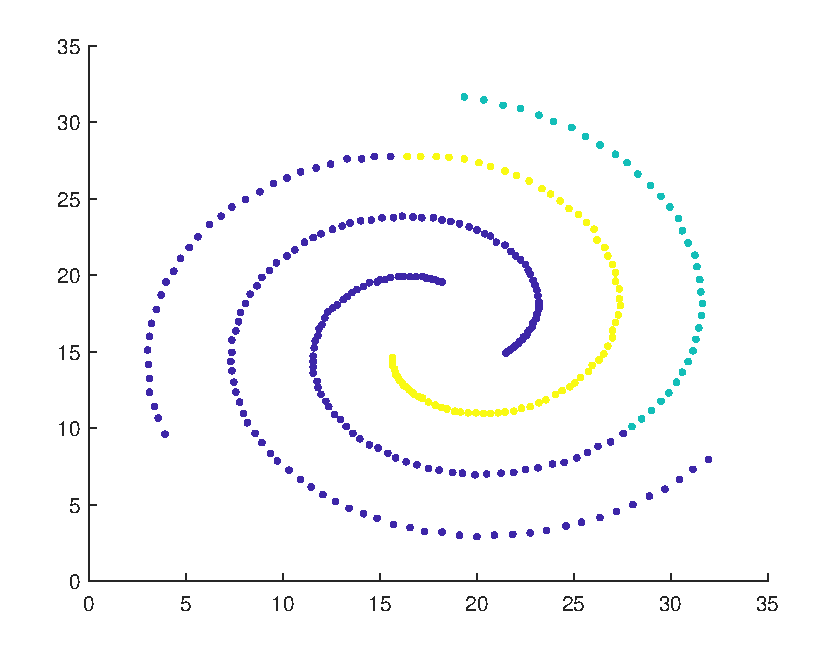
\includegraphics[scale = 0.37]{pictures/spiral_SpectralClustering_K10.pdf}}
    \subfloat[2][\(K= 20\)]{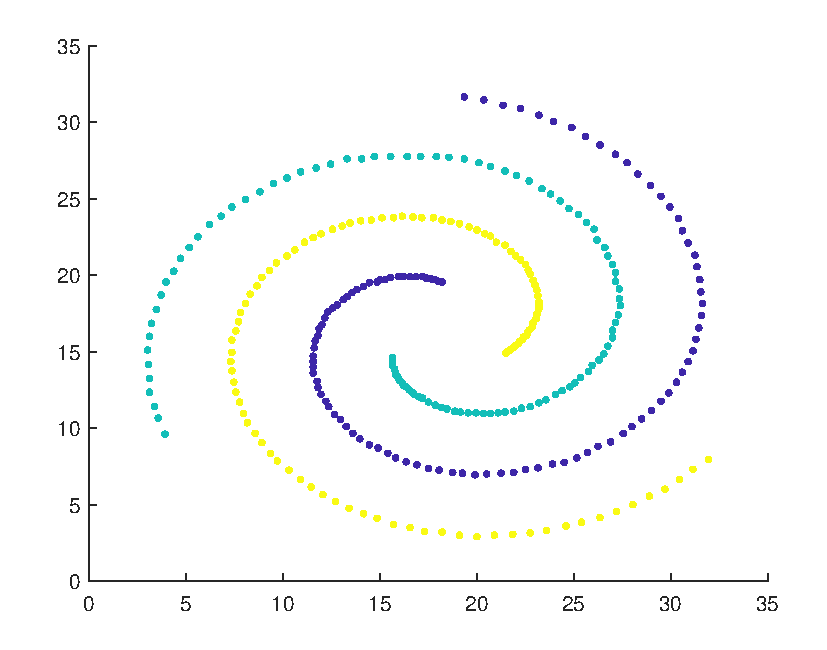
\includegraphics[scale = 0.37]{pictures/spiral_SpectralClustering_K20.pdf}}
    \subfloat[3][\(K= 40\)]{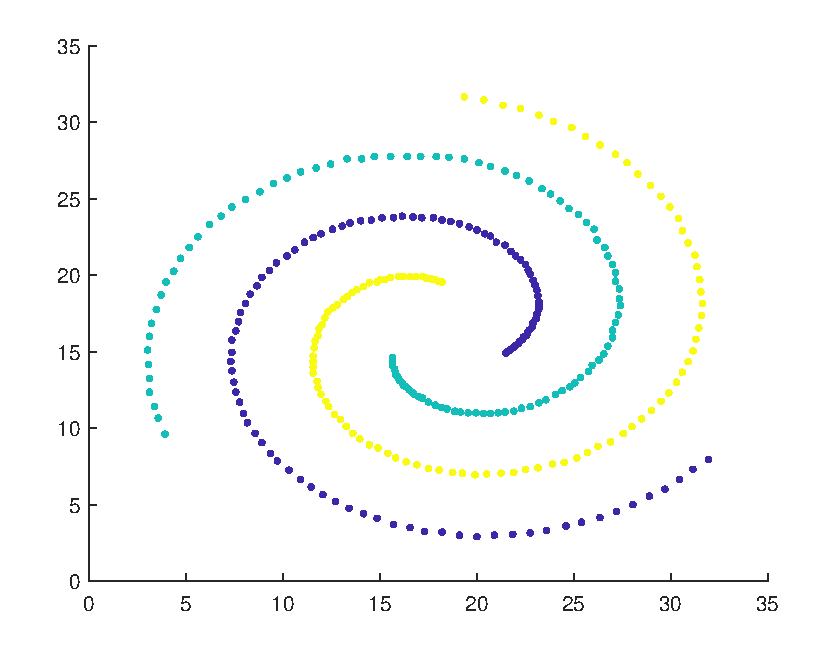
\includegraphics[scale = 0.37]{pictures/spiral_SpectralClustering_K40.pdf}}
    \caption{Spectral clustering for \texttt{spiral} data with different values of \(K\)}
    \label{spectral_spiral}
  \end{figure}
  \noindent As it is clearly visible in Figure \ref{spectral_circle}, performing spectral clustering on the \texttt{circle} data yields good results both in the case with \(K=10\) and \(K=20\). The same couldn't be said about the case \(K=40\) where the effect of pollution from one shape to another leads to poor results in terms of the proficiency of the algorithm to distinguish shapes.
  \\
  \\
  Although not every value of \(K\) yields good results for the \texttt{circle} data, the same isn't true for the \texttt{Spiral} data, where the presence of edges between spirals in the adjacency graph seems to have no effects on the fitness of the clustering, even with \(K=40\).
\section{Comparison with other clustering algorithms}
In this section we will test other clustering algorithm on the data, visualizing how they perform in comparison with the spectral clustering performed above.

\subsection{Plain \textit{Kmeans} Algorithm}
Performing the plain \textit{K-means} algorithm on our data yields poor results since the algorithm is based on euclidean distance. This is the reason it fails to recognize shapes other than balls.

\begin{figure}[H]
    \centering
    \subfloat[1][\textit{K-means} algorithm performed on \texttt{circle}]{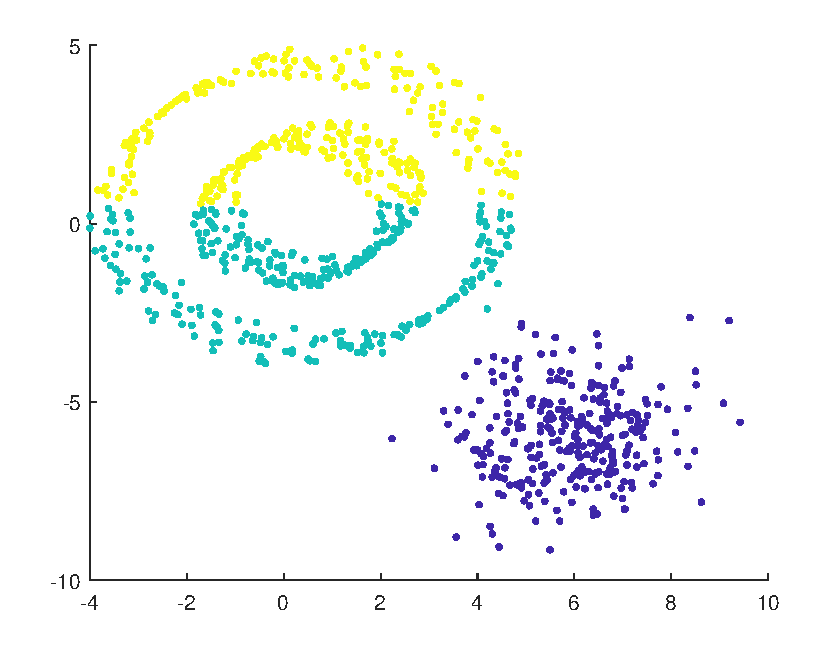
\includegraphics[scale = 0.45]{pictures/circle_Kmeans_nospectral.pdf}}
    \qquad
    \qquad
    \subfloat[2][\textit{K-means} algorithm performed on \texttt{spiral}]{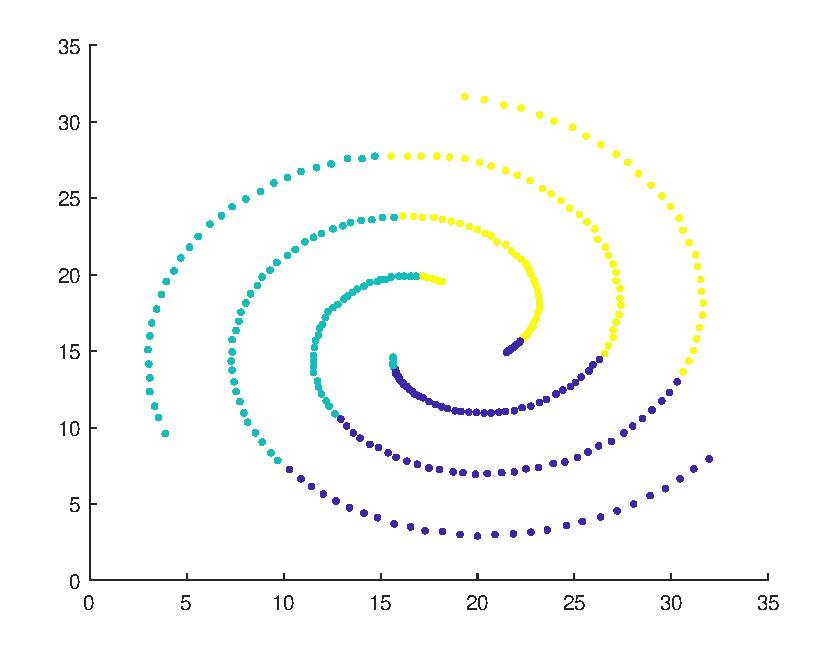
\includegraphics[scale = 0.45]{pictures/spiral_Kmeans_nospectral.pdf}}
    \caption{\textit{K-means} algorithm performed onto the datasets}
    \label{kmeans_nospectral}
  \end{figure}

  As it is clearly visible in figure \ref*{kmeans_nospectral}, the \textit{K-means} algorithm performed on spatial data is only able to recognize the cloud of points in the \texttt{circle} data since is euclidean-ball shaped. It clearly fails to recognize any other shape and this results in a very poor clustering with regard to shaped data.

  \subsection{DBSCAN algorithm}
  The DBSCAN algorithm is an "explorative" approach to clustering. Without going into details, at its core the DBSCAN algorithm populate each cluster by searching the neighborhood of each point in the cluster hence performs much better at recognizing shapes than the plain \textit{K-means} algorithm.

  \begin{figure}[H]
    \centering
    \subfloat[1][DBSCAN algorithm performed on \texttt{circle}]{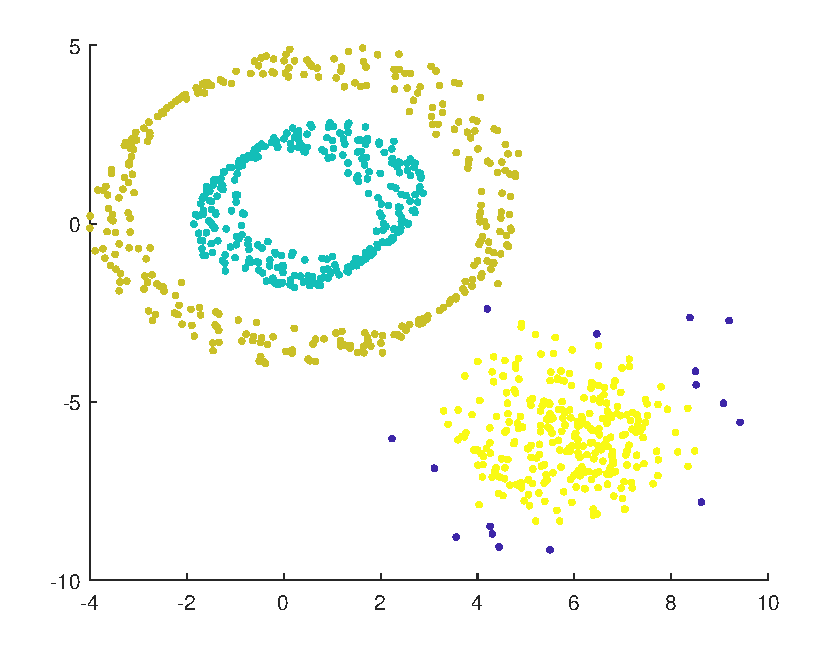
\includegraphics[scale = 0.45]{pictures/circle_dbscan_nospectral.pdf}}
    \qquad
    \qquad
    \subfloat[2][DBSCAN algorithm performed on \texttt{spiral}]{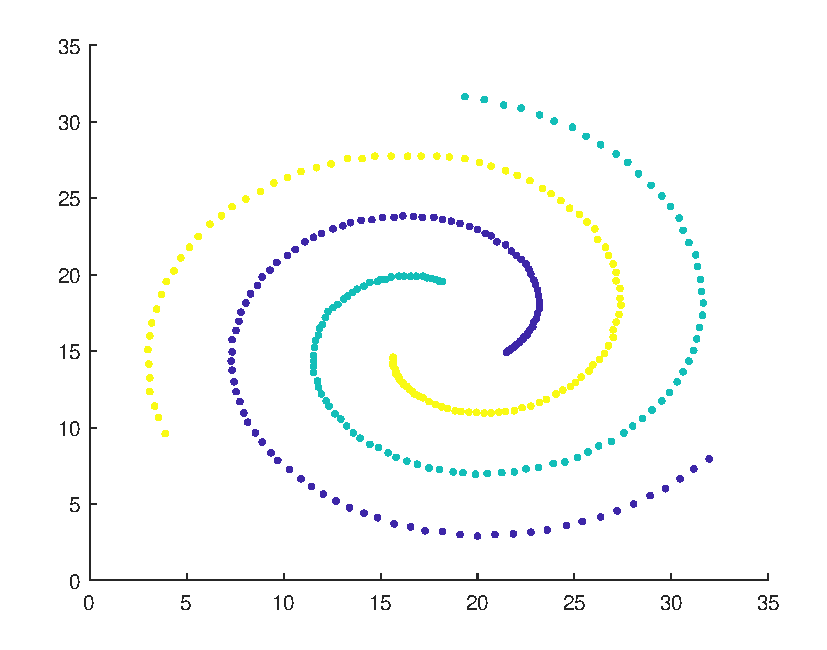
\includegraphics[scale = 0.45]{pictures/spiral_dbscan_nospectral.pdf}}
    \caption{DBSCAN algorithm performed onto the datasets}
    \label{dbscan_nospectral}
  \end{figure}

  The results of the clustering are shown in Figure \ref{dbscan_nospectral}. Those are obtained after some minor 
  %TODO

%\bibliographystyle{plain} % We choose the "plain" reference style
%\bibliography{refs} % Entries are in the refs.bib file


\end{document}